%%%%%%%%%%%%%%%%%%%%%%%%%%%%%%%%%%%%%%%%%%%%%%%%%%%%%%%%%%%%%%%%%%%%%%%%
%     LaTeX source code to approximate a Draft NIST Technical report
%	  Instructions for authors: tinyurl.com/techpubsnist 
%	DOI watermark will be added on final PDF
% 	Developed by K. Miller, kmm5@nist.gov 
%	Last updated: 22-March-2019
%%%%%%%%%%%%%%%%%%%%%%%%%%%%%%%%%%%%%%%%%%%%%%%%%%%%%%%%%%%%%%%%%%%

%%%%%%%%%%%%%%%%%%%%%%
% Template further altered by Armen Amirkhanian
% for use with UA lab courses in an effort to 
% have a standardized format for lab documents
% Last update 9-April-2020
%
% TODO:
% --Get the appendices to dynamically link, tocloft causes problems
%%%%%%%%%%%%%%%%%%%%%%

\documentclass[12pt]{article}
\usepackage{amsmath}
\usepackage{amsfonts}   % if you want the fonts
\usepackage{amssymb}    % if you want extra symbols
\usepackage{graphicx}   % need for figures
\usepackage{xcolor}
\usepackage{bm}
\usepackage{secdot}		
\usepackage{mathptmx}
\usepackage{float}
\usepackage[utf8]{inputenc}
\usepackage{textcomp}
\usepackage[hang,flushmargin,bottom]{footmisc} % footnote format
\usepackage{xspace}
%\usepackage{lineno}
\usepackage{ragged2e}
\usepackage{parskip}
\usepackage{textcomp}
\usepackage{environ}
\usepackage{multirow}
\usepackage{textgreek}

\usepackage{tikz}
\usetikzlibrary{shapes.geometric, arrows}
\tikzstyle{startstop} = [rectangle, rounded corners, minimum width=2cm, minimum height=1cm,text centered, draw=black, fill=red!20]
\tikzstyle{arrow} = [thick,->,>=stealth]

\usepackage{titlesec}
\titleformat{\section}{\normalsize\bfseries}{\thesection.}{1em}{}	% required for heading numbering style
\titleformat*{\subsection}{\normalsize\bfseries}

\usepackage{tocloft}	% change typeset, titles, and format list of appendices/figures/tables
\renewcommand{\cftdot}{}	
\renewcommand{\contentsname}{Table of Contents}
\renewcommand{\cftpartleader}{\cftdotfill{\cftdotsep}} % for parts
\renewcommand{\cftsecleader}{\cftdotfill{\cftdotsep}}
\renewcommand\cftbeforesecskip{\setlength{4pt}{}}
\addtolength{\cftfignumwidth}{1em}
\renewcommand{\cftfigpresnum}{\figurename\ }
\addtolength{\cfttabnumwidth}{1em}
\renewcommand{\cfttabpresnum}{\tablename\ }
\setlength{\cfttabindent}{0in}    %% adjust as you like
\setlength{\cftfigindent}{0in} 

\usepackage{enumitem}         % to control spacing between bullets/numbered lists

\usepackage[numbers,sort&compress]{natbib} % format bibliography 
\renewcommand{\bibsection}{}
\setlength{\bibsep}{0.0pt}

\usepackage[hidelinks]{hyperref}
\hypersetup{
	colorlinks = true,
urlcolor ={blue},
citecolor = {.},
linkcolor = {.},
anchorcolor = {.},
filecolor = {.},
menucolor = {.},
runcolor = {.}
pdftitle={},
pdfsubject={},
pdfauthor={},
pdfkeywords={}
}
\urlstyle{same}

\NewEnviron{letter}{%
\begin{quote}
\fbox{%
\begin{minipage}{\linewidth}
\setlength{\parskip}{\baselineskip}
%\letterfont
\BODY
\end{minipage}
}
\end{quote}
}

\usepackage{epstopdf} % converting EPS figure files to PDF

\usepackage{fancyhdr, lastpage}	% formatting document, calculating number of pages, formatting headers
\setlength{\topmargin}{-0.5in}
\setlength{\headheight}{39pt}
\setlength{\oddsidemargin}{0.25in}
\setlength{\evensidemargin}{0.25in}
\setlength{\textwidth}{6.0in}
\setlength{\textheight}{8.5in}

\usepackage{caption} % required for Figure labels
\captionsetup{font=small,labelfont=bf,figurename=Fig.,labelsep=period,justification=raggedright} 

%%%%%%%%%%% !!!!!REQUIRED - FILL OUT METADATA HERE !!!!!!!! %%%%%%%%%%%%%%
%%%%%%%%%%%%%%%%%%%%%%%%%%%%%%%%%%%%%%%%%%%%%%%%%%%%%%%%%%%%%%%%%%%%%%%%%%
\newcommand{\CourseNum}{CE262}
\newcommand{\CourseName}{Civil Engineering Materials}
\newcommand{\LabTitle}{Steel Tension Testing}
\newcommand{\LastUpdate}{Fall 2020}

%%%%%%%%%%%%%%%%%%%%%%%%%%%%%%%%%%%%%%%%%%%%%%%%%%%%%%%%%%%%%%%%%%%%
%   	BEGIN DOCUMENT 
%%%%%%%%%%%%%%%%%%%%%%%%%%%%%%%%%%%%%%%%%%%%%%%%%%%%%%%%%%%%%%%%%%%%
\begin{document}
	\urlstyle{rm} % Format style of \url   
%\linenumbers
\begin{titlepage}
\begin{flushright}
\LARGE{\textbf{\CourseNum{} -- \CourseName}}\\
\vfill
\Huge{\textbf{\LabTitle}}\\
    \vfill
%%%%%%%%%%%%%%%%%%%%%%%%%%%%%%%%%%%%%%%%%%%%%%%%%%%%%%%%%%%%%%%%%%%%
%	Authors - add complete list of authors, affiliations will be 
%   added on title page
%%%%%%%%%%%%%%%%%%%%%%%%%%%%%%%%%%%%%%%%%%%%%%%%%%%%%%%%%%%%%%%%%%%%
    \large Dr. Armen Amirkhanian, P.E.\\
\vfill
%%%%%%%%%%%%%%%%%%%%%%%%%%%%%%%%%%%%%%%%%%%%%%%%%%%%%%%%%%%%%%%%%%%%
%	The DOI is automated based on metadata.	
%%%%%%%%%%%%%%%%%%%%%%%%%%%%%%%%%%%%%%%%%%%%%%%%%%%%%%%%%%%%%%%%%%%%
\normalsize This work is licensed under the Creative Commons Attribution-ShareAlike 4.0 International License. To view a copy of this license, visit:
\href{http://creativecommons.org/licenses/by-sa/4.0/}{http://creativecommons.org/licenses/by-sa/4.0/}.

\includegraphics[width=0.07\textwidth]{cc.eps}
\includegraphics[width=0.07\textwidth]{by.eps}
\includegraphics[width=0.07\textwidth]{sa.eps}
\vfill

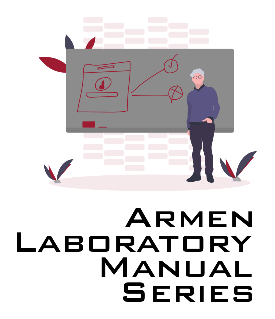
\includegraphics[width=0.3\linewidth]{Logo.eps}\\ 
 
  
\end{flushright}
\end{titlepage}

\begin{titlepage}
\begin{center}
\normalsize 
Certain commercial entities, equipment, or materials may be identified in this document in order to describe an experimental procedure or concept adequately. Such identification is not intended to imply recommendation or endorsement by The University of Alabama or the listed authors, nor is it intended to imply that the entities, materials, or equipment are necessarily the best available for the purpose.\\
\vfill
Any opinions or recommendations are solely those of the author(s) and do not represent the official view or policy of The University of Alabama.
\end{center}
\begin{flushright}
\vfill
\normalsize 
This document was last updated in \textbf{\LastUpdate} and should contain \textbf{\pageref{LastPage}} pages of content exclusive of these title pages, abstract, and other front matter. If the document appears to be incomplete, please contact the author(s).\\
\vfill
Engineering is the art of modelling materials we do not wholly understand,\\into shapes we cannot precisely analyse,\\so as to withstand forces we cannot properly assess,\\in such a way that the public has no reason to suspect the extent of our ignorance.\\
\textit{A.R. Dykes}
\end{flushright}
\end{titlepage}
%%%%%%%%%%%%%%%%%%%%%%%%%%%%%%%%%%%%%%%%%%%%%%%%%%%%%%%%%%%%%%%%%%%%
%   Start front matter - page number starts with "i"
%%%%%%%%%%%%%%%%%%%%%%%%%%%%%%%%%%%%%%%%%%%%%%%%%%%%%%%%%%%%%%%%%%%%
\pagenumbering{roman}
\section*{Abstract}
\normalsize Steel is an important material used in civil engineering. While we often make the design process easy by using different grades of steel and simplifying assumptions, it is still critical to understand the behavior of the material as it undergoes elastic and plastic deformations. Since we are dealing with a relatively homogeneous material, unlike portland cement concrete or asphalt concrete, we can easily characterize the material properties of steel alloys using small specimens and we have the added benefit of not having to deal with aging effects.

\vfill
\section*{Keywords}
\normalsize steel; tension; elastic modulus; yield strength.\\
\pagebreak
%%%%%%%%%%%%%%%%%%%%%%%%%%%%%%%%%%%%%%%%%%%%%%%%%%%%%%%%%%%%%%%%%%%%
%   Table of Contents is required
% 	List of Tables & Figures required if more than 5 tables/figures
%%%%%%%%%%%%%%%%%%%%%%%%%%%%%%%%%%%%%%%%%%%%%%%%%%%%%%%%%%%%%%%%%%%%
\begin{center}
\tableofcontents
\pagebreak
\listoftables
\listoffigures
\end{center}
\pagebreak
\section*{Required Specifications}
The following specifications are required to complete this laboratory exercise:
\begin{description}
\item[ASTM A370] Standard Test Methods and Definitions for Mechanical Testing of Steel Products
\end{description}

The following specifications are optional, but they are listed here in the event more information is needed to complete the laboratory exercise:
\begin{description}
\item[ASTM E8] Standard Test Methods for Tension Testing of Metallic Materials
\end{description}
\pagebreak
%%%%%%%%%%%%%%%%%%%%%%%%%%%%%%%%%%%%%%%%%%%%%%%%%%%%%%%%%%%%%%%%%%%%
%   Start body of text - page number starts with "1"
%%%%%%%%%%%%%%%%%%%%%%%%%%%%%%%%%%%%%%%%%%%%%%%%%%%%%%%%%%%%%%%%%%%%
\section{Steel Tension Testing}
\label{sec:intro}
\pagenumbering{arabic}
\normalsize 
This laboratory exercise is a tension test but we will be calculating much more than a simple tensile strength of steel. By looking at the entirety of the stress-strain behavior, we will be able to calculate the elastic modulus, yield strength, and ultimate tensile strength, among other properties.

\subsection{Objectives}
\label{ssec:headingscap}
At the completion of this lab exercise section, you will have satisfied the following objectives:
\begin{enumerate}
    \item Observe a steel tension test
    \item Perform an analysis of data that is output from commercial testing equipment
    \item Perform calculations necessary to determine the elastic modulus, yield strength, and ultimate tensile strength
\end{enumerate}

\subsection{Learning Outcomes}
At the completion of this lab exercise, you should be able to:
\begin{itemize}
    \item understand the stress-strain behavior of steel alloys used in civil engineering applications
    \item understand the quantitative calculations needed to determine specific material properties
    \item understand how knowledge of the alloy does not equate to knowing the strength and durability of a steel alloy
    \item present calculated values in a useful and professional manner
\end{itemize}

\pagebreak
\subsection{Procedure}
The majority of this laboratory exercise already has the procedure ``handled''. You are not expected to understand how to program the testing frame to run the test nor are you expected to run the experiment by yourself.

\subsubsection{Before Testing}
Prior to running the tension test on your steel specimen, you will need to measure the geometry. A set of calipers are available so that you can accurately take the measurements necessary. Two important measurements are:
\begin{itemize}
    \item Cross-sectional area of the portion that will fracture
    \item Gauge\footnote{You'll see ``gage'' and ``gauge'' length used interchangeably. They mean the same thing.} length of the extensometer
\end{itemize}

If you are completing this lab virtually, the pertinent measurements will be contained within the datafile from the test runs.

\subsubsection{Execution}
The execution of the actual test method will be handled by the instructor. Not only is the equipment expensive and sensitive, it is dangerous. The frame can crush your fingers and keeping going without a second thought.

\subsubsection{After Testing}
After your specimen has been tested to failure, note the type of fracture (i.e. cup and cone, planar, etc). The type of failure provides a visual and qualitative indication of the modulus and failure mode of the alloy. Talk with your instructor during your observation of the fracture surface to learn more about what to expect in your data analysis.

\newpage
\subsection{Data Analysis}
You will need to calculate three properties (Fig. \ref{fig:prop}) for this laboratory exercise:
\begin{itemize}
    \item Elastic modulus (i.e. Young's modulus)
    \item Yield strength
    \item Ultimate tensile strength
\end{itemize}

The elastic modulus is the slope of the linear portion of the stress-strain curve and is easily found by using a linear fit or some other slope calculation. The yield strength is a little more unique and we actually will draw a line, with the same elastic modulus that we calculate for the specimen, but start at 0.2\% strain and go up until we hit our data. This is commonly called the 0.2\%-offset yield strength. Finally, the ultimate tensile strength is the maximum stress that our specimen ever sees, which is usually different than the stress at the point of fracture.

\begin{figure}[h]
    \centering
    \includegraphics[width=0.7\textwidth]{true1.eps}
    \caption{Example of the three material properties being calculated. Your stress/strain curve may not look exactly like this and that is okay.}
    \label{fig:prop}
\end{figure}

The following sections will describe how to perform the calculations specific to the equipment that was used in the laboratory exercise. You will ``show your work'' graphically and will not need to provide step-by-step calculations. At all times, keep in mind some of these ballpark numbers to know if you are determining the values correctly:
\begin{itemize}
    \item Elastic modulus\footnote{ksi: kilo pounds per square inch. 1 ksi = 1,000 psi.}: 20,000--40,000 ksi
    \item Yield strength: 40,000--120,000 psi
    \item Ultimate tensile strength: must be greater than yield strength
\end{itemize}

\subsubsection{Initial Data Import}
The first thing you will need to do is import the data from the testing machine into Excel. This is as simple as opening the file in Excel! Upon opening the file, there will be some content at the top of the data indicating the geometry of the specimen. There will also be columns of data:
\begin{itemize}
    \item[\textbf{Crosshead}] This describes the distance that the fixture, which is hold the specimen, has moved during the test.
    \item[\textbf{Load}] This is self-explanatory and has already been made a positive number, even though it is indicating a tensile load.
    \item[\textbf{Time}] This is recorded so that you could verify that the test machine loaded the specimen at the correct testing rate. You will not need to worry about this.
    \item[\textbf{Extensometer}] This is the direct reading from the clip-on extensometer. Note that it is not directly giving you strain, but rather a direct calculation of the distance it is opening.
\end{itemize}
We will need to convert the load into a stress. We can do that by dividing the load by the cross-sectional area of the specimen. Be sure to check your units to make sure you are consistent! 

You will also need to convert the extensometer values into a strain. We know the extensometer is measuring over its gauge length, so the strain is calculated by simply dividing the current extensometer reading by the gauge length. If we were to multiply, that resulting number by 100, we would get the strain as a percentage. This will be helpful later on.

Now we need to have a serious discussion about true stress/strain and engineering stress/strain. You may have heard these terms in other classes. As we load our specimen, the cross-sectional area will change due to several factors. Thus, we should \textit{technically} recalculate the stress at each step with the ever changing cross-sectional area. The effect of doing this is shown in Fig. \ref{fig:true}. 

There is a significant difference in the stresses that are calculated after the specimen starts yield. In civil engineering, we are content to use the engineering stress/strain values. There are several reasons why. The first and foremost is the simplicity. It can be extremely difficult to calculate the reduction in area as the specimen is loaded to its fracture point. Another practical consideration is that we never design for ultimate tensile strength or fracture strength. We, in civil engineering, only design for the yield strength. Up to the yield point, the true stress/strain and engineering stress/strain are identical as the specimen has not seen any appreciable permanent deformation and a resulting reduction in cross-sectional area.

\begin{figure}[h]
    \centering
    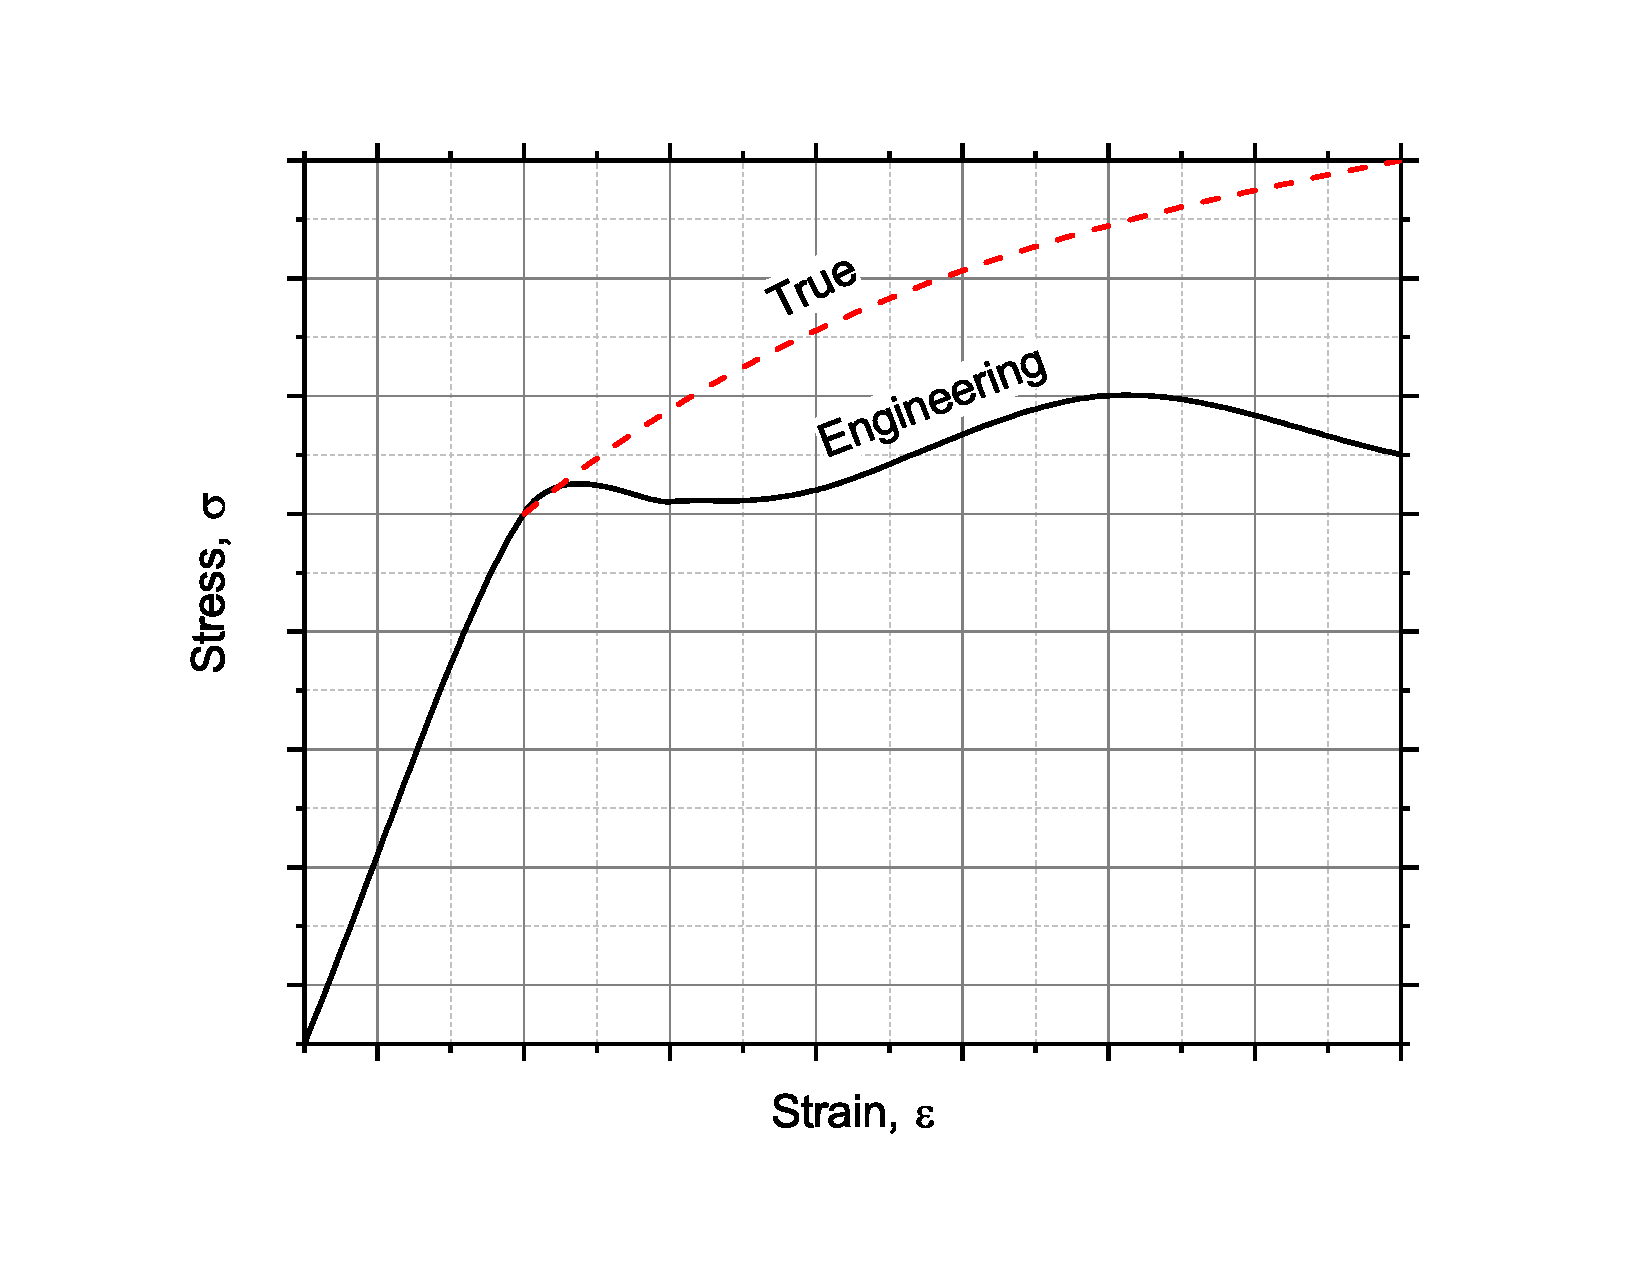
\includegraphics[width=0.7\textwidth]{true.eps}
    \caption{Example of true stress/strain as compared to engineering stress/strain. Most civil engineering applications use engineering stress/strain due to simplicity and relevancy.}
    \label{fig:true}
\end{figure}

With that out of the way, we can plot our data to see what happened with our steel specimens. To assist you in checking your calculations, your data should plot as shown below (Fig. \ref{fig:real}). The plot only shows data that the extensometer captured before it was removed from the specimen. You will have to manually locate the point in the data where this occurs. It is usually fairly easy to determine this as the extensometer values level off for several readings then suddenly jump around as the gauge is removed.

\begin{figure}
    \centering
    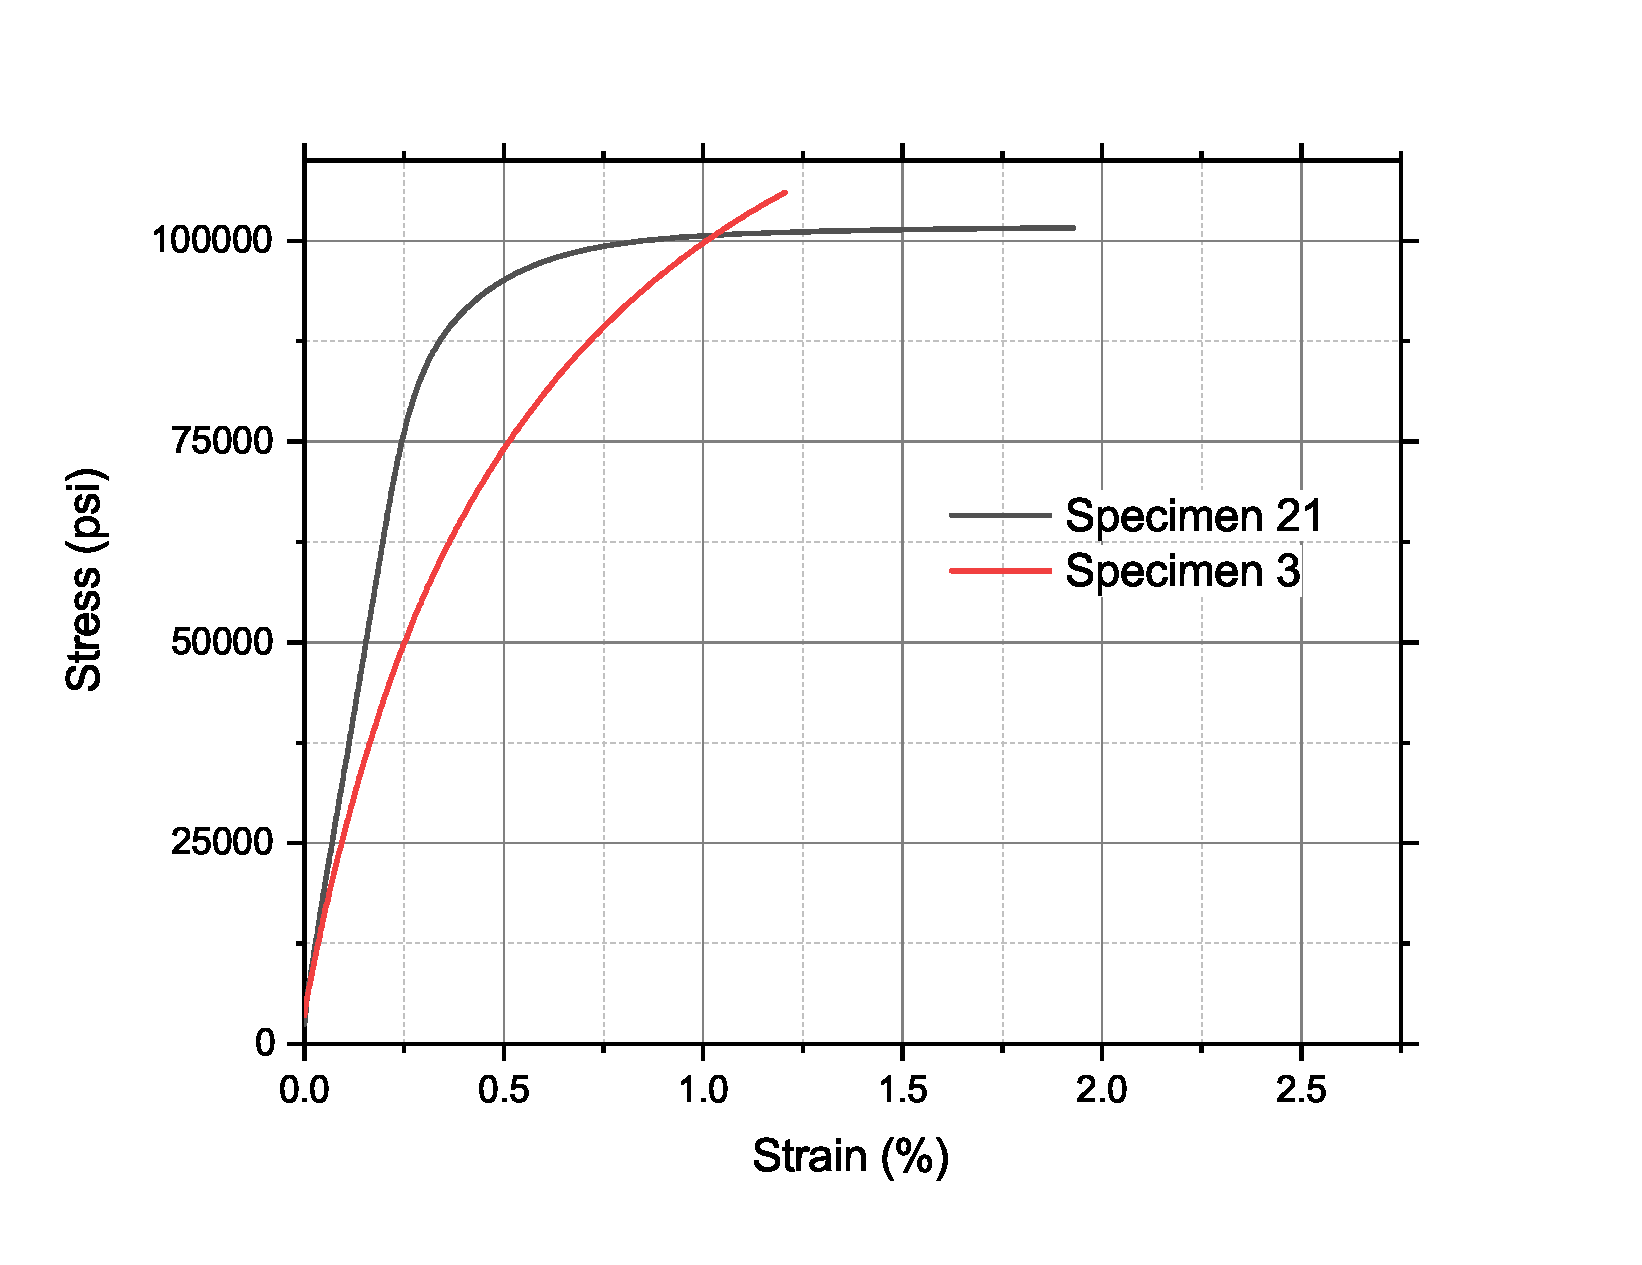
\includegraphics[width=0.7\textwidth]{real.eps}
    \caption{\textbf{Data from Fall 2020 laboratory exercise.} If your plot does not match this (values), you have a calculation error. You may have slightly more or less data plotted depending on where you decided to cutoff the data with the extensometer removal.}
    \label{fig:real}
\end{figure}

\subsubsection{Elastic Modulus Calculation}
You will need to find the slope of the linear portion of the data. Similar to calculating the elastic modulus with concrete, we do not want to start at zero as there will be some initial seating effects. For this lab, visually select a linear portion (Fig. \ref{fig:elastgraph}) of the stress/strain curve and find the slope.

\begin{figure}[h!]
    \centering
    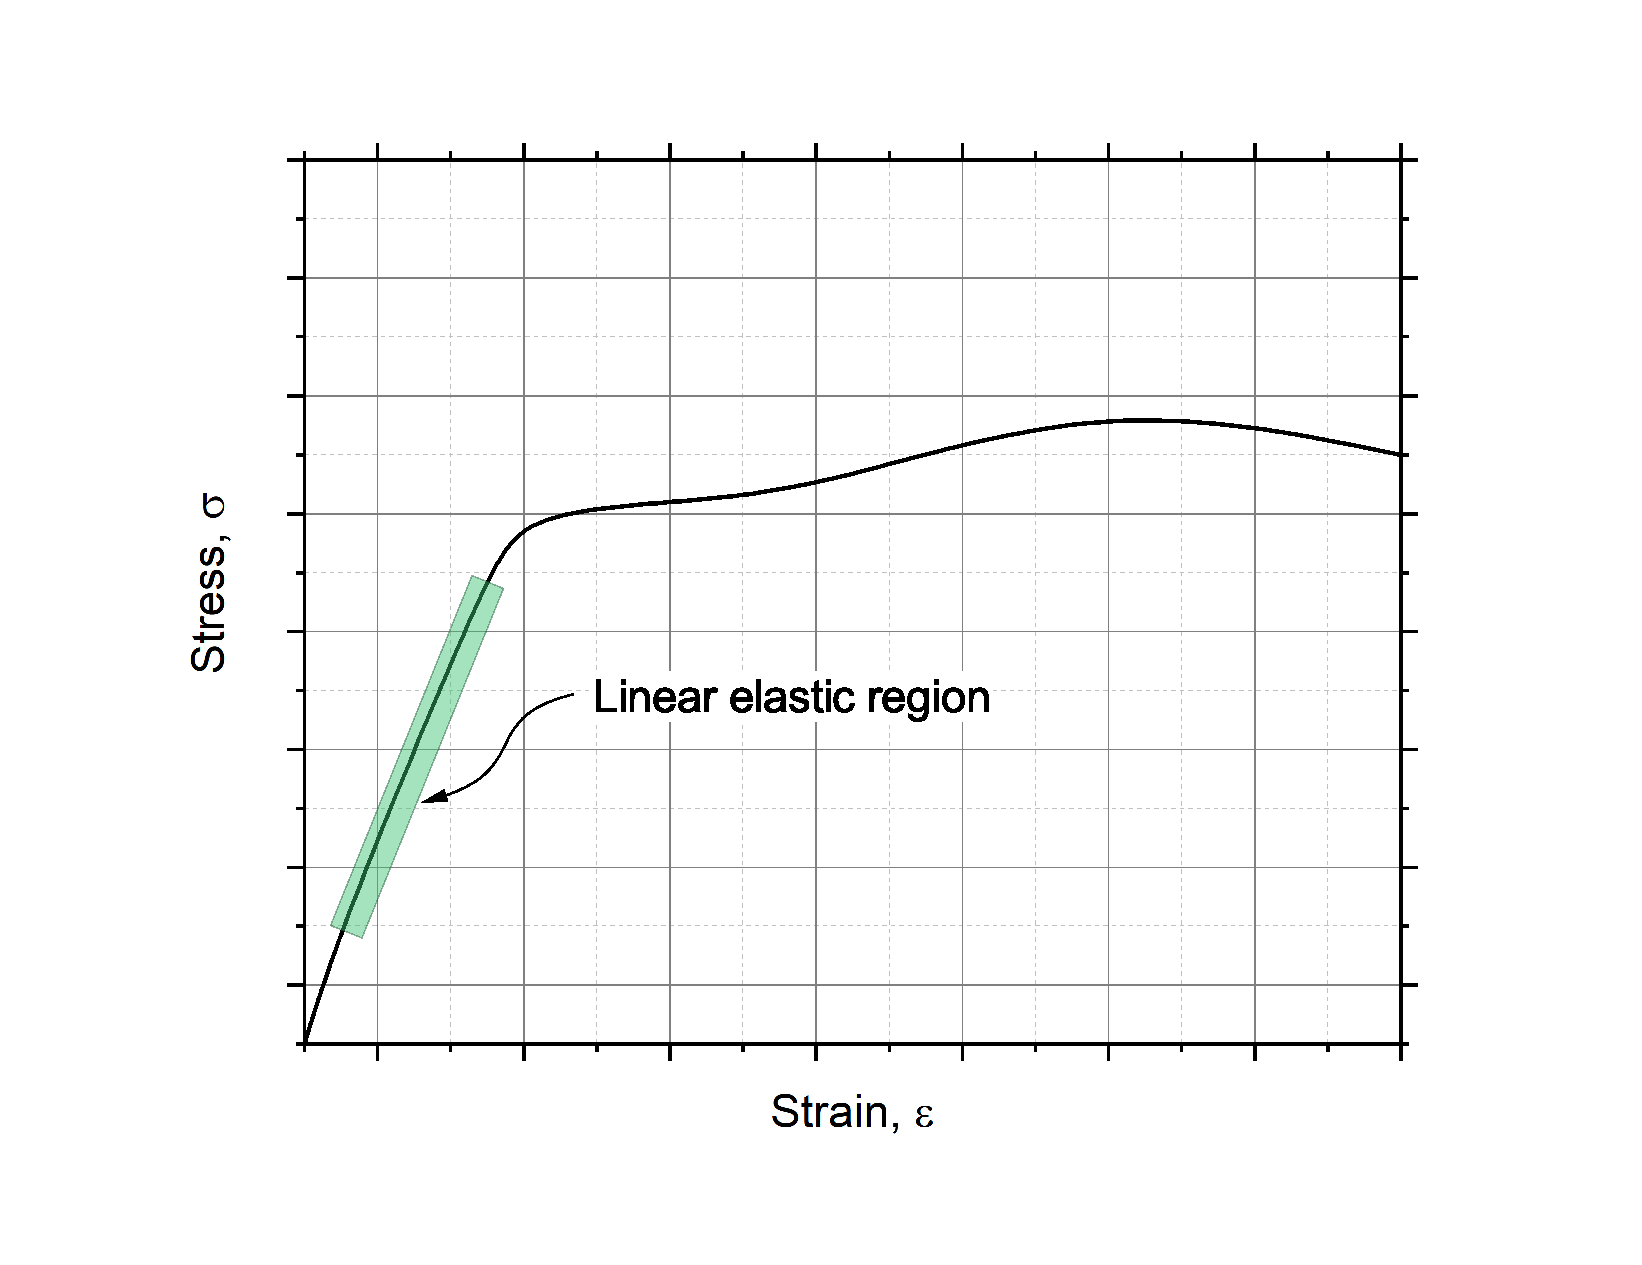
\includegraphics[width=0.7\textwidth]{offset3.eps}
    \caption{Visual determination of the linear elastic portion of the data. Note that the region does not extend to the start of the test.}
    \label{fig:elastgraph}
\end{figure}

There are several methods that can be used to find the slope. The most reliable is to manually select the data that is in the linear elastic range, plot it, then apply a linear fit to it (Fig. \ref{fig:trend}). In this example, the slope of the linear fit is 29,000,000 psi which is a reasonable value for steel. The intercept value has no useful meaning for us in this laboratory exercise.

\textbf{Note for Fall 2020: Specimen 3 had an abnormality with the extensometer during the test. Your calculated elastic modulus for this data set will be extremely low. Please report the value you calculate but understand it is not representative of the true modulus.}

\begin{figure}[h!]
    \centering
    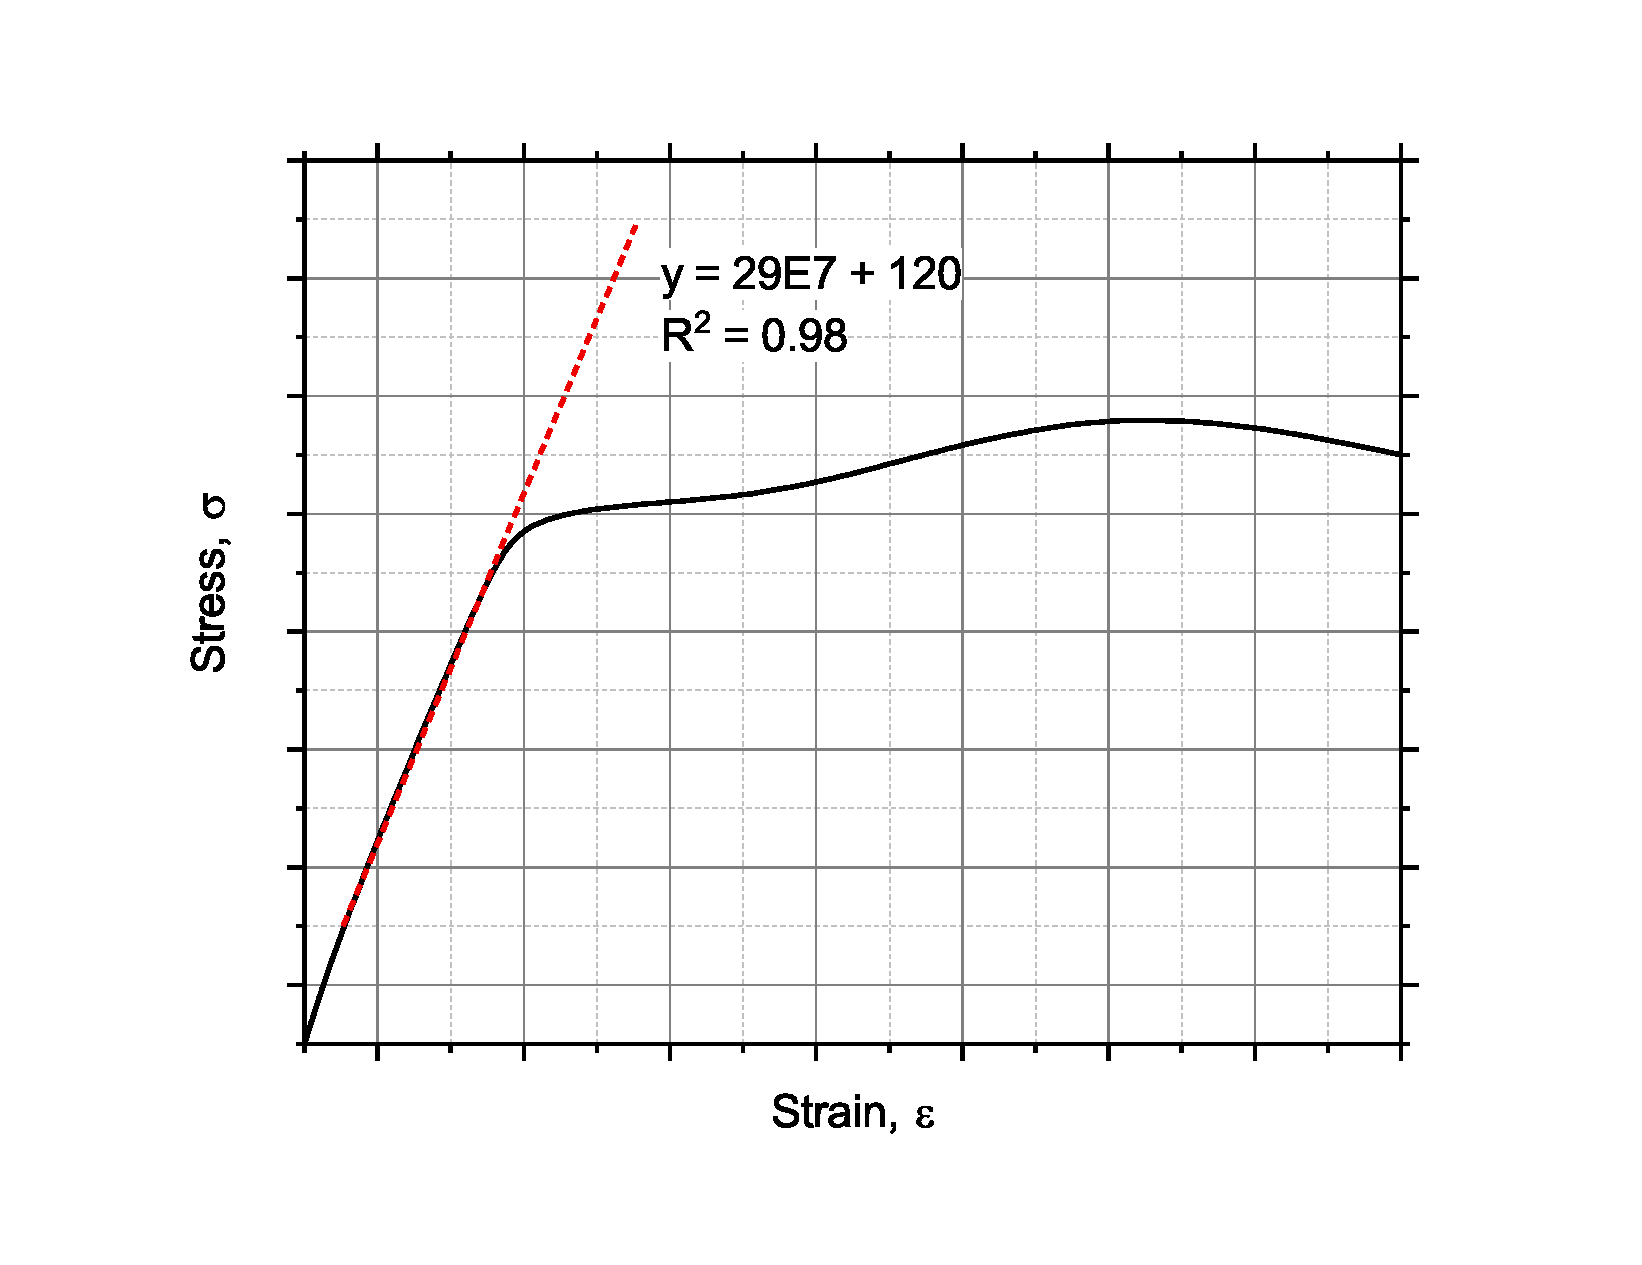
\includegraphics[width=0.65\textwidth]{offset4.eps}
    \caption{Linear portion of the data plotted with the resulting linear trendline and equation. Keep track of your units!}
    \label{fig:trend}
\end{figure}

\subsubsection{Yield Strength Calculation}
The yield strength is a much more difficult value to calculate because without expert knowledge of fracture mechanics and metal deformation theory, it is a type of guessing game. In order to have a consistent method to measure the yield strength, the idea of an offset yield strength has been developed. Based on the offset chosen, a straight line will be drawn up, using the same elastic modulus of the actual data, until the line ``hits'' the data. The point at which this line intersects the actual data is considered to be the yield strength (Fig. \ref{fig:prop}). For steel alloys, we commonly use 0.2\% strain as the offset point. Thus, we commonly refer to the yield strength for steel alloys as the 0.2\%-offset yield strength\footnote{For steel alloys, if no offset is reported with a yield strength, you can safely assume an implied 0.2\% offset.}.

You should never hand draw a 0.2\%-offset line but rather calculate it. If you think about what you are doing, you'll see it is a fairly straightforward process. You are trying to draw a straight line with a slope of $E$. You want it to pass through 0.2\% strain (and zero stress). The equation of a straight line is $y=mx+b$. You have all the pieces neccessary to calculate and plot the straight line for the offset method!

\subsubsection{Ultimate Tensile Strength Calculation}
This is the easiest of the three listed properties to calculate. You will report the maximum stress applied to the specimen at any time during testing. Unlike the modulus and yield strength calculations, we need to consider the entire dataset. Since we are only looking for a peak stress, it does not matter if the extensometer was on the specimen or not.

\pagebreak
\section{Deliverables}
For this laboratory exercise, you will need to submit a single data sheet. You will put both specimens onto the same page. Unlike the previous submissions, there is no example document for this data sheet. Use the experience from creating the other data sheets to guide you in presenting the information from this lab in a clear and professional manner. Your single page submission, at a minimum, should include:
\begin{itemize}
    \item Plot of stress/strain data for both specimens. Include on the plot the calculated 0.2\%-offset yield strength lines to show how you obtained the yield strength. DO NOT DRAW A LINE ON THE PLOT. You must calculate it and plot it alongside the data.
    \item Specimen dimensions necessary for the calculations
    \item Brief description of the two specimens (i.e. visual appearance, prior damage/treatment, etc)
    \item Table of material properties that includes elastic modulus, 0.2\%-offset yield strength, and ultimate tensile strength
    \item Any notes or comments that would be useful for the reader
    \item Any fields (i.e. name, specification, etc) that are neccessary to provide the reader information about the technician and process
\end{itemize}

A large part of this exercise is professional formatting. You will likely spend more time making the page(s) look good than performing the actual calculations and this is okay! Professional engineers will typically use software specifically designed to make nice sheets. However, there are still some firms and engineers that do it manually. Most of the time the entire page is created in MS Excel due to the insane number of rows and columns needed. Here are some DOs and DON'Ts to help guide you in making a professional submission:

\begin{itemize}
    \item DO be consistent with decimal places and where applicable, follow the ASTM/ACI rules for number of decimal places
    \item DO indicate units properly
    \item DON'T include extraneous fields that have values of ``N/a'' or similar
    \item DON'T use a font size smaller than 10pt
    \item DON'T use shading (i.e. shading alternating rows)
    \item DON'T use a cover page
\end{itemize}

%\section*{References}
%\addcontentsline{toc}{section}{References}
%\bibliographystyle{techpubs}
%\bibliography{References}

%%%%%%%%%%%%%%%%%%%%%%%%%%%%%%%%%%%%%%%%%%%%%%%%%%%%%%%%%%%%%%%%%%%%
%   Please use the techpubs BibTeX style when compiling bibliography, or follow the instructions on tinyurl.com/techpubsnist to format your .bib / .bbl file appropriately.
%%%%%%%%%%%%%%%%%%%%%%%%%%%%%%%%%%%%%%%%%%%%%%%%%%%%%%%%%%%%%%%%%%%%
\pagebreak
\section*{Appendix A: Photos of Fracture Surface}
\label{AppendixA}
\addcontentsline{toc}{section}{Appendix A: Photos of Fracture Surface}

\renewcommand\thefigure{A\arabic{figure}}
\setcounter{figure}{0}


\begin{figure}[h]
    \centering
    \includegraphics[width=0.6\textwidth]{ST-4.jpg}
    \caption{Photo of untreated steel specimen. Notice the pronounced necking in the region of the failure. This necking behavior is seen in the failures of ductile alloys.}
    \label{fig:app1}
\end{figure}

\begin{figure}[h]
    \centering
    \includegraphics[width=0.6\textwidth]{ST-1.jpg}
    \caption{Photo of heat treated steel specimen. Notice the lack of any significant necking. While there is slight necking visible, it is nowhere near as pronounced as the specimen in Fig. \ref{fig:app1}.}
    \label{fig:app2}
\end{figure}

\begin{figure}[h]
    \centering
    \includegraphics[width=1\textwidth]{ST-2.jpg}
    \caption{Side-by-side comparison of the two specimen's fracture faces. Note the heat treated specimen (left) has an extremely flat fracture face while the untreated specimen (right) has a rough fracture face. In addition, the heat treated sample has a slightly different color and texture on the fracture face than the untreated specimen. This is significant but outside the scope of the course.\\ \textit{Legos used with permission from my kids.}}
    \label{fig:app3}
\end{figure}

\begin{figure}[h]
    \centering
    \includegraphics[width=1\textwidth]{ST-5.jpg}
    \caption{Close-up view of the fracture face of the untreated specimen. The geometry of the fracture face is a cup-and-cone. Notice that the left side (cone) fits into the right side (cup). This failure mode is unique and expected of ductile alloys.\\ \textit{Legos used with permission from my kids.}}
    \label{fig:app4}
\end{figure}

\begin{figure}[h]
    \centering
    \includegraphics[width=1\textwidth]{ST-6.jpg}
    \caption{Close-up view of the cup portion of the untreated specimen fracture face. This failure mode is unique and expected of ductile alloys.\\ \textit{Legos used with permission from my kids.}}
    \label{fig:app5}
\end{figure}
    
    


%\pagebreak

%\section*{Appendix A2: Fine Aggregate Datasheet}
%\label{AppendixB}
%\addcontentsline{toc}{section}{Appendix A2: Fine Aggregate Datasheet}
%\begin{center}
%    \includegraphics[width=1\linewidth]{Fine.eps}
%\end{center}

%\pagebreak

%\section*{Appendix B: Example Concrete Mixture Form}
%\label{AppendixB}
%\addcontentsline{toc}{section}{Appendix B: Example Concrete Mixture Form}
%\begin{center}
%    \includegraphics[width=1\linewidth]{1608_v11_1.eps}
%\end{center}


%\pagebreak
%\section*{Appendix B: Change Log}
%\addcontentsline{toc}{section}{Appendix B: Change Log}
%This document was originally created on April 9, 2020. Any changes will be documented in this appendix.

\end{document}
%%%%%%%%%%%%%%%%%%%%%%%%%%%%%%%%%%%%%%%%%%%%%%%%%%%%%%%%%%%%%%%%%%%%
%   When referring to references in the text parenthetically, 
%	use the form “[1].” For example, “As Jones and Smith have shown [1];”
%	 however, when a reference is referred to non-parenthetically, use the form 
%	“. . . Ref. [1] . . .” (except at the beginning of a sentence where
%	“Reference [1] . . .” is the correct form).
%%%%%%%%%%%%%%%%%%%%%%%%%%%%%%%%%%%%%%%%%%%%%%%%%%%%%%%%%%%%%%%%%%%%

%%%%%%%%%%%%%%%%%%%%%%%%%%%%%%%%%%%%%%%%%%%%%%%%%%%%%%%%%%%%%%%%%%%%
%   Section references are “Sec. X”.
% 	“Section X” is used at beginning of sentence. 
%%%%%%%%%%%%%%%%%%%%%%%%%%%%%%%%%%%%%%%%%%%%%%%%%%%%%%%%%%%%%%%%%%%%

%%%%%%%%%%%%%%%%%%%%%%%%%%%%%%%%%%%%%%%%%%%%%%%%%%%%%%%%%%%%%%%%%%%%
%   Equation references are “Eq. (X)”.
% 	“Equation (1) is used at beginning of sentence.
%	Equations are numbered (#) on the right, per the standard LaTeX format
%%%%%%%%%%%%%%%%%%%%%%%%%%%%%%%%%%%%%%%%%%%%%%%%%%%%%%%%%%%%%%%%%%%%

%%%%%%%%%%%%%%%%%%%%%%%%%%%%%%%%%%%%%%%%%%%%%%%%%%%%%%%%%%%%%%%%%%%%
%   Tables should appear after they are mentioned in the text. 
%	Superscripted letters (a, b, c, etc.) should be used for table footnotes.
%%%%%%%%%%%%%%%%%%%%%%%%%%%%%%%%%%%%%%%%%%%%%%%%%%%%%%%%%%%%%%%%%%%%

%%%%%%%%%%%%%%%%%%%%%%%%%%%%%%%%%%%%%%%%%%%%%%%%%%%%%%%%%%%%%%%%%%%%
%   Figure references are “Fig. X”.
% 	“Figure X” is used at beginning of sentence. 
% 	Figures should appear after they are mentioned in the text.
%	Figures must have embedded alternate text or “alt text” in order 
%	to comply with Section 508 accessibility standards. 
%%%%%%%%%%%%%%%%%%%%%%%%%%%%%%%%%%%%%%%%%%%%%%%%%%%%%%%%%%%%%%%%%%%%